\documentclass[A4paper, 12pt]{article}
\usepackage{fancyhdr}
\usepackage{graphicx}
\usepackage{booktabs}
\usepackage{pdfpages}
\usepackage[spanish]{babel}
\pagestyle{fancy}
\lhead{Vulcano 2.0:  Un Nuevo Comienzo}
\rhead{v2.03 SPA}
\cfoot{\thepage}
\renewcommand{\headrulewidth}{0.4pt}
\renewcommand{\footrulewidth}{0.4pt}
\begin{document}
\title{Vulcano 2.0: A New Beginning}
\author{The Vulcano Team}
\date{\today}
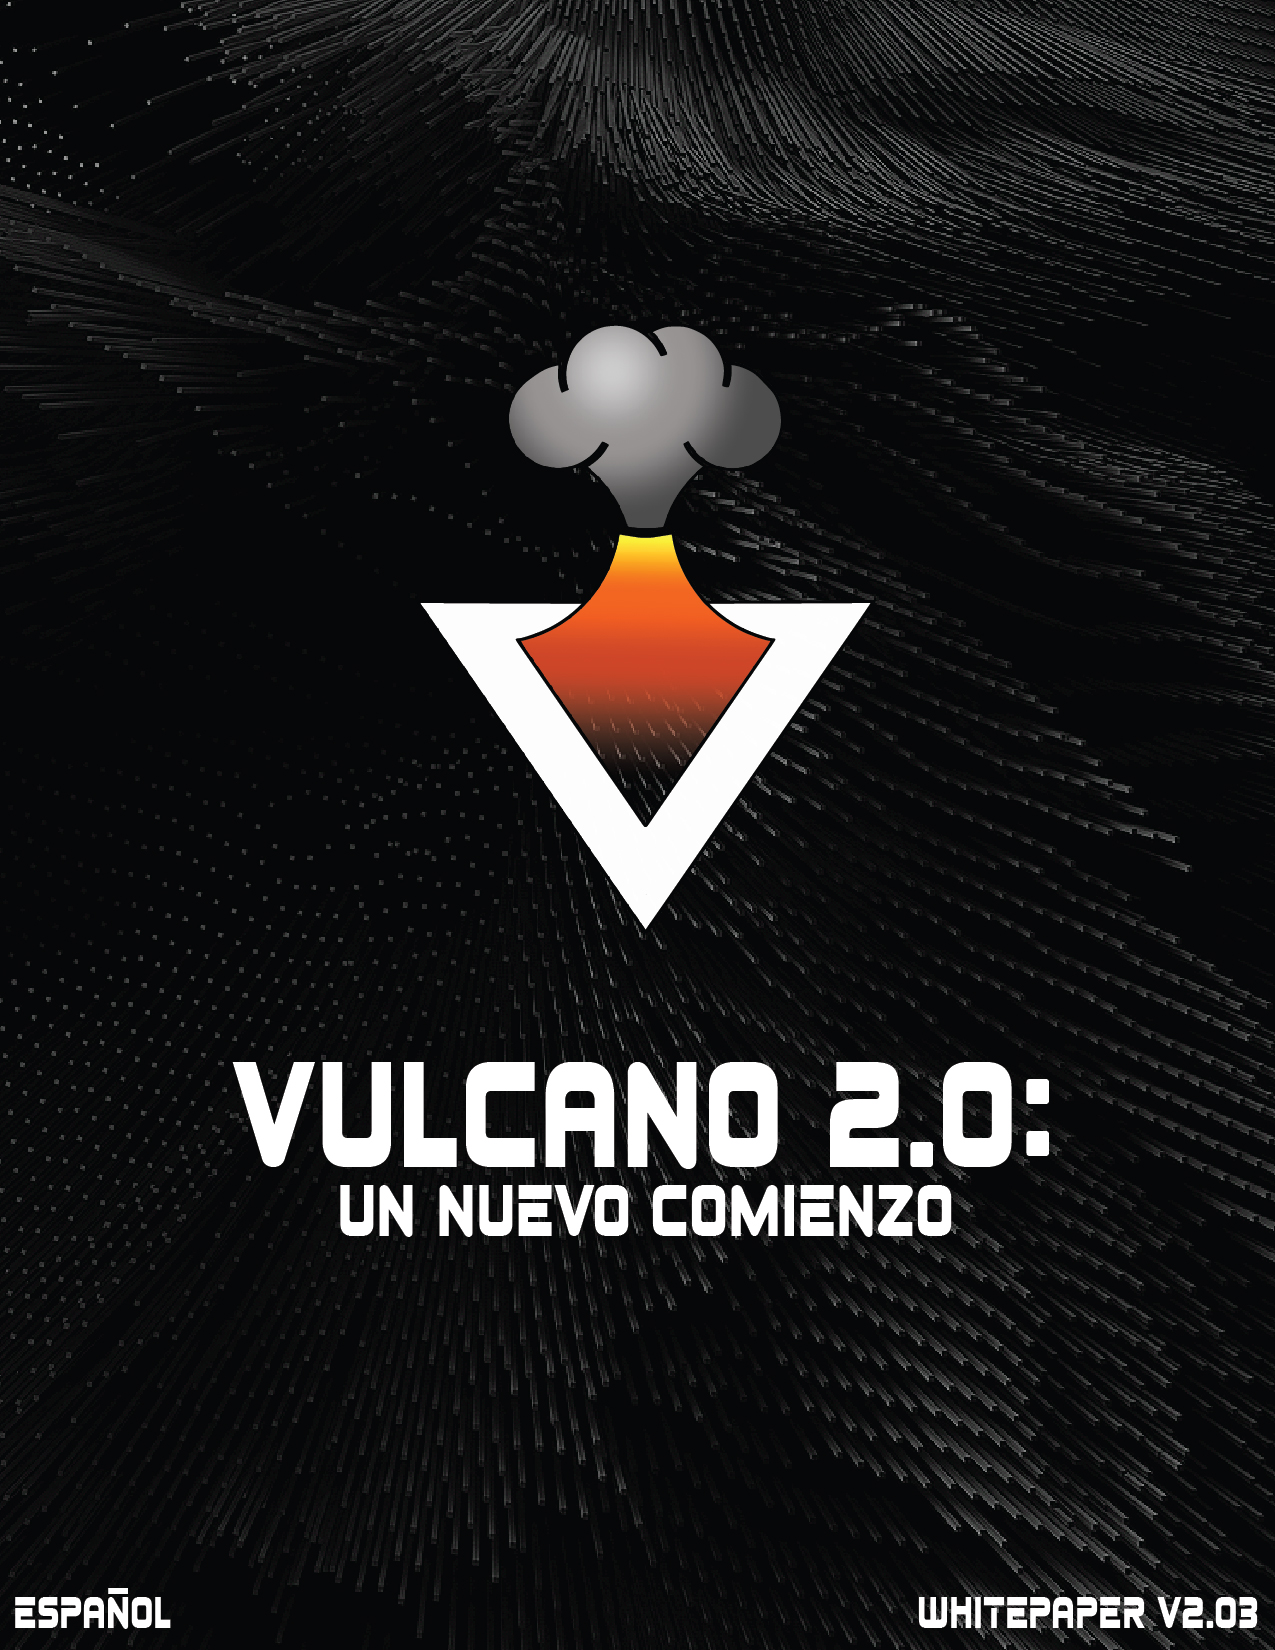
\includepdf[pages=1]{COVER-SPA.pdf}
\newpage
\tableofcontents
\newpage
\section{Introducción}

Vulcano (ticker: VULC) es una moneda orientada a la comunidad creada originalmente a finales de 2017 por un equipo de desarrollo completamente ausente.   Inicialmente, se concibió como una "moneda de alto riesgo" con un rendimiento anual del 950\%. Sin embargo, debido a varios errores por parte del equipo de desarrollo inicial, la tasa real fue más cercana al 320.000\%.   Esto pasó desapercibido hasta que un miembro de la comunidad calculó esta tasa efectiva al examinar la cadena de bloques del Bloque Génesis1 .   Una vez que se descubrió esta debilidad fundamental, el nuevo equipo de Vulcano, compuesto por miembros de la comunidad, se unió para rescatar el proyecto Vulcano tanto a nivel técnico como filosófico a través de una reconstrucción completa y el desarrollo de un caso de uso real. Este documento técnico establece una estrategia para una mejora total de Vulcano y un relanzamiento de la moneda recientemente actualizada como un medio para financiar la exploración e investigación geotérmica.

En lugar de simplemente arreglar el problema de la tasa de porcentaje con Vulcano, hemos elegido actualizar completamente la moneda a una nueva base de código.    Con el fin de modernizar mejor el Vulcano Core, el equipo de Vulcano ha decidido utilizar Bulwark como base de código.  Bulwark se basa en PIVX, que a su vez está basado en la popular criptomoneda DASH. Esta decisión crítica nos dará la capacidad de implementar la funcionalidad de masternodos, la gobernanza y, finalmente, permitir la integración de nodos de hardware para soportar el ecosistema de Vulcano.  Al hacerlo, crearemos un sistema de gobernanza y apropiación de monedas y seguridad de red más verdaderamente descentralizado.

Este documento también describirá los planes futuros para la legitimación de Vulcano a través de la creación de la Fundación Vulcano, una entidad 501(c)3 sin fines de lucro planificada con sede en los Estados Unidos que permitirá a Vulcano desarrollarse de manera madura y para comenzar a conectarse y entrar en negociaciones con el resto del mundo de los negocios. Esto es especialmente importante ya que el caso de uso a largo plazo de Vulcano exige la adquisición de una cartera de propiedad intelectual a través del mecanismo de investigación que se explica a continuación. Mediante la creación de una cartera de propiedad intelectual a través de la financiación de la investigación en universidades e instituciones de investigación de todo el mundo. La Fundación Vulcano nos permitiría aprovechar mejor esta propiedad intelectual. Este es un paso absolutamente crítico que permitirá al proyecto descentralizado Vulcano interactuar y conectarse con los mundos centralizados de negocios y el mundo académico.

Este documento también establecerá los porcentajes planificados de honorarios de gobernanza que irán directamente a la financiación de la investigación geotérmica con el fin de avanzar en la ciencia y obtener propiedad intelectual para traer más fondos a la Fundación Vulcano para desarrollos futuros y para proporcionar fondos para subvenciones adicionales.

Lo que no encontrarás en este documento son promesas falsas y sin fundamento sobre el futuro de la cadena de bloques de Vulcano.  Vulcano se esfuerza por la innovación y el crecimiento sin hacer promesas que no se puedan cumplir, en lugar de eso, dedicaremos nuestros esfuerzos a la investigación y al avance del desarrollo tecnológico. Toda la tecnología de cadena de bloques mencionada en este documento ya se ha demostrado y se activará a su debido tiempo.  Creemos que es hora de que las comunidades de criptomonedas comiencen a actuar de una manera que sea consistente con el potencial de negocios que traen a la mesa, y que no se necesitan afirmaciones falsas sobre la tecnología cadena de bloques para construir un caso comercial para el uso de la tecnología existente.  Los desarrolladores, los líderes del equipo y las propias comunidades deben comprender que para ser aceptados por las comunidades empresariales y académicas en general, debemos estar dispuestos a seguir sus reglas hasta cierto punto y hacer un uso efectivo de lo que tenemos antes de presentar ideas sobre la tecnología de cadena de bloques no probada antes de que se haya desarrollado, probado o planeado.  Si bien puede haber avances en la tecnología de la cadena de bloques para Vulcano en el futuro, su lanzamiento no vendrá con meses de fanfarria y marketing, pero solo se hablará una vez que ya se haya desarrollado.  Creemos que este método de desarrollo "submarino" es mejor para la moneda porque limita la inversión especulativa y permite la construcción de una base estable para la plataforma en el futuro.

Nuestro objetivo es convertir a Vulcano en una de las principales fuentes de fondos para la investigación de sostenibilidad en el futuro y, finalmente, construir un ecosistema empresarial en torno a esta tecnología.

\section{Agradecimientos}
Vulcano no hubiera sido posible sin los trabajos previos de los equipos Bitcoin, Peercoin, Blackcoin, Talkcoin, Dash, PIVX y, lo más importante, Bulwark. Como la nueva encarnación de Vulcano es una bifurcación modificada de Bulwark, se han tomado prestado varias secciones directamente de su hoja blanca para las funcionalidades que incluiremos, pero que no serán modificadas desde la base de código existente. Nosotros, el Vulcano Team, pensamos que sería más transparente incluir estas secciones como las que existen en el documento de Bulwark en lugar de reescribirlas y fingir que son completamente originales. Si bien es importante que nosotros, como comunidad, desarrollemos casos de uso sólido y estructuras comerciales que funcionen para el mundo en general, el espíritu de código abierto detrás de la criptomoneda debe ser protegido y mantenido en el futuro. La humanidad, como un todo, se beneficia del intercambio de la información y estamos orgullosos de contribuir a este creciente cuerpo de conocimiento. Es en este mismo espíritu que ofreceremos las tecnologías desarrolladas con financiamiento a través de la Fundación Vulcano a las naciones que contribuyen al ecosistema de Vulcano.

\section{Una breve introducción a las criptomonedas}
Si bien las propuestas de tecnología de registro contable distribuida se remontan a finales de la década de 1980, no fue hasta el lanzamiento de un documento sobre un oscuro tablero de anuncios de criptografía titulado “Bitcoin: Un sistema de efectivo electrónico punto a punto” por un escritor bajo el seudónimo de Satoshi Nakamoto que nació una verdadera cadena de bloques. Una cadena de bloques funciona marcando las transacciones secuencialmente y bloqueándolas en "bloques" que son validados por varios métodos para que no puedan manipularse.   Bitcoin y muchas otras criptomonedas operan basándose en la "Prueba de trabajo", lo que significa que usan el poder computacional como recurso de escasez dentro de su red.

Sin embargo, como Vulcano se enfoca en la sustentabilidad y la investigación en el campo de la energía, este método no sostenible es antitético a nuestros esfuerzos por aumentar la sostenibilidad.   Por lo tanto, hemos elegido operar sobre la base de una "prueba de participación", donde el recurso de escasez en la red son los propios tokens.  Además, con el lanzamiento del Vulcano mejorado lanzado 30 días después de la publicación de este documento técnico, también tendremos masternodos, que son una versión un poco más avanzada del método de prueba de trabajo en el que las computadoras de todo el mundo mantienen la red, pero también tienen una carga computacional simple para el propósito. A partir de ahora, esta carga computacional es apenas mayor que la operación de un simple monedero, pero nos gustaría utilizar esta red en el futuro para computación distribuida para la industria de energía renovable para el funcionamiento de problemas de física y computación computacional. Esta es una adición importante al plan a largo plazo para Vulcano, ya que los departamentos geofísicos y geotérmicos de las universidades de investigación generalmente no están tan bien financiados como otros campos más glamorosos y, por lo tanto, les resulta más difícil obtener tiempo de ciclo en las computadoras grandes para ejecutar sus simulaciones.

Además, desde la perspectiva del consumidor, con un tiempo de bloque de 90 segundos, consenso de masternodos y bloque de transacciones, un cronograma de emisiones estabilizado y controlado y participación ecológica, Vulcano aspira a ser una criptomoneda verdaderamente rápida y funcional que tenga un impacto real en el mundo, pero también es una opción fuerte para los consumidores y entusiastas de la criptomoneda.

\section{El Nuevo Vulcano}
\subsection{Detalles de la nueva cadena de bloques Vulcano}

\begin{table}[h]
\centering
\begin{tabular}{@{}ll@{}}
\toprule
Ticker & VULC \\ \midrule
Algoritmo & NIST5 \\
Puerto RPC & 62541 \\
Puerto P2P & 62543 \\
Bloque espaciado & 90 segundos \\
Algoritmo de dificultad & Dark Gravity Wave v3.0 \\
Tamaño de bloque & 1MB \\
Madurez de minería/acuña & 67 Bloques ($\sim$100 minutos) \\
Confirmación & 6 Bloques ($\sim$9 minutos) \\
Circulación (1 Año) & 246,194,250 \\
Circulación (1 Años) & 421,126,225 \\
Período de PoW & nHeight 60 \\
Período de PoS & nHeight 61 \\
Protocolo de soporte & IPV4, IPV6, TOR \\
PoS & Blackcoin v3.0 PoS \\ \bottomrule
\end{tabular}
\end{table}

\subsection{Manteniendo la comunidad unida}
Vulcano fue originalmente concebido como una moneda comunitaria y esta es una idea en la que creemos de todo corazón.  Como moneda comunitaria, sabemos que la mejor manera de servir al desarrollo del proyecto es servir a la comunidad a la que le debemos nuestra existencia. Continuaremos nuestras lluvias, concursos y otras actividades basadas en la comunidad. También promoveremos la discusión y la exploración de los límites del Ecosistema de Vulcano.  En todos los foros, mantendremos nuestra política de cero tolerancias hacia el acoso de los recién llegados, los usuarios y otras comunidades de criptomonedas. Vulcano cree que hay suficiente espacio en el mundo de la criptomoneda que podemos y debemos esforzarnos por conectar y sinergizar en lugar de destruir otros proyectos. Si bien comprendemos que existe un grado de competencia afable entre los adherentes de varias plataformas de criptomoneda, nos gustaría mantener todas las interacciones positivas.

\subsection{Desarrollando la Capacidad Empresarial}
Al momento de escribir, ha habido una afluencia de criptomonedas que utilizan una base tecnológica similar. Si bien la tecnología subyacente es sólida, a menudo un examen más profundo de sus especificaciones y los parámetros de cadena de bloques revela prácticas menos justas.  En otros casos, la implementación tecnológica es deficiente, pero la comunidad no está suficientemente informada sobre los problemas para poder determinar esto y participar en un proyecto fundamentalmente poco sólido.

Desafortunadamente, el Vulcano original podría haber caído fácilmente en esta categoría, que es una de las principales razones por las cuales el nuevo equipo de Vulcano está dando la vuelta al proyecto en su totalidad. Creemos que las criptomonedas deben tener aplicaciones comerciales reales y que esta tecnología no debe usarse solo para generar ingresos especulativos para un pequeño número de titulares que actúan antes de que el mercado comprenda lo que realmente está sucediendo. Con demasiada frecuencia hemos visto a los desarrolladores construir una mala moneda, bombearla con publicidad glamorosa, y luego abandonar el proyecto y dejar a la comunidad como bagholders. Es por eso que creemos en la transparencia y la responsabilidad, y estableceremos la base comercial necesaria para hacer negocios reales con los mundos criptográficos y no criptográficos.

Como tal, estableceremos varias organizaciones comerciales formales para facilitar estas interacciones.  La primera y más importante es la organización sin fines de lucro 501(c)3 que estableceremos con el propósito de dirigir fondos hacia iniciativas geotérmicas y de investigación en ciencias de la tierra. Esta organización será responsable del mantenimiento de cualquier propiedad intelectual y de marca.

También habrá una serie de LLCs establecidas para requisitos locales alrededor del mundo. Muchos intercambios de criptomonedas requieren una entidad comercial local y, al establecer una red de LLC, eso se puede proporcionar. Esta red le dará a la Fundación Vulcano y a la comunidad de Vulcano la capacidad de realizar negocios en cualquier parte del mundo sin perder la capacidad de responder a las necesidades locales y los requisitos legales.
 
\subsection{Mantenimiento de la comunidad}
La comunidad VULC es el factor más importante detrás del éxito a largo plazo del proyecto, y su capacidad para influir significativamente en el futuro de la moneda y el desarrollo tecnológico de nuestras áreas clave es primordial. Como nuestro objetivo primordial es avanzar en la investigación sobre la sostenibilidad a través del mecanismo de la energía geotérmica casi ilimitada que está bajo nuestros pies, hemos puesto en marcha planes para proporcionar fondos a los investigadores que trabajan en estas áreas.

Como tal, al final de nuestros primeros seis meses, en el bloque 172801, tenemos la intención de activar los bloques de Eruption de presupuesto en la red. Estos bloques Eruption, pagados mensualmente, permitirán a la comunidad ejercer un control significativo sobre la investigación que Vulcano financia, el desarrollo de la presencia de la marca y los asuntos de la comunidad.  Retrasar la activación de este sistema en aproximadamente seis meses desde el lanzamiento nos dará tiempo para desarrollar el marco subyacente necesario para una experiencia de usuario positiva y permitir que el sistema se estabilice a partir de los cambios en la tasa de emisión de tokens con una reducción de 320.000\% a algo mucho más razonable.

Además, se agregará una estructura de gobierno del 10\% a todas las recompensas por bloque que se utilizarán de forma transparente y rastreable para financiar la investigación geotérmica. A medida que esto continúe, utilizaremos un proceso de varias fases para crear y enviar propuestas además de aquellas que seleccionamos a través de nuestros propios esfuerzos.  Para que una propuesta sea aceptada, cada paso en el proceso de selección deberá completarse.  Como creemos que la sabiduría y el conocimiento pueden provenir de una amplia variedad de lugares, alentamos a la Comunidad Vulcano a idear sobre las tecnologías que rodean a la Energía Geotérmica. Estas propuestas e ideas se reunirán y podrán ser votadas y discutidas por el resto de la comunidad antes de ser exploradas con mayor profundidad a nivel académico. Esperamos que la comunidad de Vulcano pueda atraer expertos geotérmicos de todo el mundo para contribuir a este proceso de ideación.

\subsection{Tasa de emisión de Vulcano}
A continuación, se muestra las recompensas de bloque y la tasa de emisión de la cadena de bloques Vulcano.
\begin{table}[h]
\centering
\begin{tabular}{@{}ccccc@{}}
\toprule
Mes & Número de bloque & Recompensa de Bloque & Emitido & Total \\ \midrule
0 & 0-1 & 95,000,000 & 95,000,000 & 95,000,000 \\
1-6 & 2 a 172800 & 500 & 86,396,500 & 181,396,500 \\
7-12 & 172801 a 345600 & 375 & 64,797,750 & 246,194,250 \\
13-18 & 345601 a 518400 & 281.25 & 48,598,313 & 294,792,563 \\
19-24 & 518401 a 691200 & 210.94 & 36,448,734 & 331,241,297 \\
25-30 & 691201 a 864000 & 158.20 & 27,336,551 & 358,577,848 \\
31-36 & 864001 a 1036800 & 118.65 & 20,502,413 & 379,080,261 \\
37-42 & 1036801 a 1209600 & 88.99 & 15,376,810 & 394,457,071 \\
43-48 & 1209601 a 1382400 & 66.74 & 11,532,607 & 405,989,678 \\
49-54 & 1382401 a 1555200 & 50.06 & 8,649,456 & 414,639,133 \\
55-60 & 1555201 a 1728000 & 37.54 & 6,487,092 & 421,126,225 \\
61+ & 1728001 al Infinito & 18.77 & Continúa & Continúa \\ \bottomrule
\end{tabular}
\end{table}

\subsection{Trabajando para derrotar la centralización}

Existen varios problemas endémicos de los ecosistemas de cadena de bloques que existen actualmente. Estos problemas, si bien existen en diferentes dominios, se pueden describir como una sobrecentralización de una manera u otra.

El primer tipo de centralización que debe eliminarse es el hecho de que la gran mayoría de los tokens o monedas existentes están en manos de especuladores. Esto lleva a oscilaciones de precios completamente irracionales a medida que diversos actores intentan manipular los mercados mientras que los especuladores desinformados que buscan la próxima "luna" compran y venden posiciones rápidamente.  Si bien esto tiene poco o ningún impacto en el desarrollo real, crea una actitud dentro de la comunidad de que las fluctuaciones de los precios de alguna manera determinan o reflejan la salud fundamental del proyecto, cuando están completamente desconectados. Este problema de centralización en manos de los especuladores conduce a la volatilidad y un alto grado de riesgo. Uno de nuestros objetivos es gestionar esto en la mayor medida posible.

El segundo tipo de centralización es la centralización geográfica en términos de los Servidores Privados Virtuales sobre los que se configuran normalmente los masternodos. Con los servicios que ofrecen hosting de masternodos barato, existe una tendencia para que la comunidad despliegue una gran cantidad de nodos en un solo proveedor de servicios, lo que significa que un único evento imprevisto puede eliminar un gran porcentaje de la red, lo que genera vulnerabilidades.

Una solución a este problema hermanado de la sobrecentralización es el Ecosistema de Investigación Vulcano. Como la Fundación Vulcano financia investigaciones en el dominio geotérmico, se espera que adquiera una cartera de propiedad intelectual. Nuestro plan es ofrecer esta propiedad intelectual a un costo muy bajo a cualquier institución o nación que acuerde alojar nodos de hardware de Vulcano2. De esta forma, estas instituciones contarán con un conjunto de herramientas tecnológicas para utilizar como componentes básicos de sus propias tecnologías por el simple costo de desplegar masternodos en sus propios sistemas o en un nodo de hardware de Vulcano. Esto aumentará en gran medida la distribución geográfica de los masternodos de Vulcano y al mismo tiempo disminuirá el número de tokens que flotan en la comunidad y estarán disponibles para la especulación.

También creemos que es importante que el token de Vulcano se distribuya lo más ampliamente posible. De hecho, creemos que la mayoría de los proyectos de criptomonedas pequeñas que tienen grandes porcentajes de tokens en manos de un pequeño número de titulares introduce un grado peligroso de centralización en el proyecto. Como tal, tenemos la intención de presentar planes en el futuro para incentivar la descentralización y la fragmentación de monederos grandes y recompensar a aquellos que tienen un número menor de masternodos.  Esto será discutido en una fecha posterior.

Como el equipo de Vulcano es un firme defensor del desarrollo de código abierto, nos gustaría mantener este modo de negocio casi de código abierto para tantas áreas como sea posible.  Por supuesto, todos los códigos fuente estarán siempre disponibles para su inspección, pero también nos gustaría proporcionar un cuerpo de propiedad intelectual para usarlo lo más económicamente posible.

\section{Características de Vulcano}
\subsection {Masternodos}
Los masternodos, tomados colectivamente, son una red descentralizada de computadoras que sirven a la red Vulcano. Realizan funciones de red importantes y reciben una parte de las recompensas en bloque. Además de cumplir con estas funciones básicas de red, ayudan estabilizando el suministro de monedas, procesando acciones y asegurar la red.   Los masternodos requieren 50.000 VULC y conocimientos técnicos modestos para operar.  Cualquier monedero que controle 50.000 VULC puede configurar un masternodo.

El equipo de Vulcano tiene planes a largo plazo para introducir varios tipos de nodos que otorgarán recompensas en función de su contribución a una red computacional útil. De esta manera, el desafío de la "prueba de trabajo" puede eludirse en los cálculos que se realizan no son cálculos arbitrarios para asegurar la red, sino cálculos funcionales para contribuir al avance de las ciencias relacionadas con la sostenibilidad. Se dará a conocer más información sobre esta propuesta a medida que se produzcan nuevos desarrollos.

\subsection{Ofuscación / mezcla de monedas}
Como el nuevo código de Vulcano Core se basa en Bulwark, también ofrece ofuscación, que se realiza de forma descentralizada y facilitada por la red de masternodos. Esto proporciona una capa adicional de privacidad en las transacciones. Aunque no es perfectamente anónima, la confusión a través de la mezcla de nodos es muy superior a la transacción estándar de Bitcoin.  Por ejemplo, todas las transacciones de Bitcoin son transparentes y se pueden seguir fácilmente a través de la cadena de bloques.   Para Vulcano, un actor nefasto necesitaría controlar al menos el 50\% de los masternodos operativos para tener una probabilidad mayor de 0.5\% de anonimizar una sola transacción que se mezcló con 8 rondas de Ofuscación.  Esta característica importante proporciona un alto nivel de anonimato para los usuarios de VULC que eligen obstruir sus transacciones.   Si bien no está íntimamente conectado con el caso de uso final del proyecto Vulcano, proporciona un grado de usabilidad del consumidor que mejora su valor en relación con otros proyectos en la etapa de criptomonedas.

\subsection{SwiftTX}
SwiftTX proporciona masternodos con autorización de bloque y consenso para las transacciones. Cuando se envía una transacción a la red, un grupo de masternodos validará la transacción.  Si esos masternodos alcanzan el consenso sobre la validez de la transacción, se bloqueará para su posterior introducción en la cadena de bloques, aumentando en gran medida la velocidad de transacción en comparación con los sistemas convencionales (como los tiempos de bloque de 10 minutos de Bitcoin con múltiples confirmaciones). SwiftTX hace posible que se realicen transacciones múltiples antes de que un bloque en la red se extraiga con las mismas entradas.  Este sistema se basa en InstantSend de Dash.

\subsection{Sporks}
La nueva red Vulcano emplea el mecanismo de horquilla de fases múltiples que se introdujo en Bulwark y se conoce como "sporking". Esto permitirá a la red VULC implementar nuevas características a la vez que se minimizan las posibilidades de una bifurcación de la red no deseada durante el despliegue. Los cambios de Spork se pueden implementar a través de la red y se pueden activar y desactivar según sea necesario sin requerir actualizaciones de software de nodo. Esta característica es extremadamente útil y permite que la red reaccione rápidamente a las vulnerabilidades de seguridad sin requerir la entrada de usuarios individuales para actualizar manualmente su código de monedero.

\subsection{Masternodos TOR y IPV6}
Vulcano permitirá al usuario ejecutar su nodo completo o masternodo desde una dirección de onion o una dirección IPV6. Hemos estado trabajando para agregar nodos de TOR completos tanto para fortalecer la red de TOR como para la experiencia de usuario de Bulwark que opera en modo solo TOR. Una característica única del soporte de TOR es capaz de operar su masternodo como un servicio TOR oculto.  Los nodos TOR permiten a los usuarios con conexiones a Internet estables operar los masternodos fuera de su red doméstica sin las implicaciones de privacidad de revelar su ubicación o los peligros de exponer su red doméstica al potencial de ataque o compromiso.
 
\section{El Futuro}
\subsection{Nodo de hardware seguro de Vulcano}
Los elementos clave del equipo de Vulcano están trabajando actualmente con un fabricante especializado de productos electrónicos de consumo de alta gama para desarrollar nodos de hardware seguros que pueden implementarse globalmente para proporcionar la descentralización de la red y un mayor grado de seguridad. Los usuarios podrán conectar esto a su red doméstica y configurar mediante una interfaz de usuario web. Las funciones que pretendemos iniciar con fácil configuración de masternodo completamente onionizado (o nodo completo) utilizando servicios ocultos de TOR para aquellos con conexiones a Internet estables.

De acuerdo con el espíritu de descentralización, todos los códigos fuente estarán disponibles para la comunidad para el ensamblaje en el hogar, pero también estarán disponibles en un modelo estándar.  Estos nodos también serán los nodos que están distribuidos por la Fundación Vulcano en nuestro esfuerzo por aumentar la distribución geográfica y el bloque de monedas mediante la implementación de nodos estáticos.

\subsection{La Tienda Vulcano}
De preocupación inmediata es la creación de un caso de uso del mundo real para Vulcano. El primer ejemplo de esto será un mercado de bienes digitales que opere a partir de la cadena de bloques Vulcano. Si bien esto inicialmente será para productos digitales de fuera de la comunidad, como los códigos de Steam y las tarjetas de regalo, se planea gastar para convertirse en un mercado de igual a igual basado en Vulcano.

\subsection{Telegram y Discord Bots}
El alma de cada proyecto de cadena de bloques es la comunidad, y una de las mejores formas de servir a la comunidad es dándoles una forma de comunicarse y usar el token. El equipo de Vulcano financiará la creación de bots para varios servicios de chat que permitirán a las personas compartir sus VULC fácilmente con el resto del mundo. Al facilitar este flujo libre de Vulcano, podemos mejorar la utilidad a la vez que involucramos y hacemos crecer a la comunidad.

\section{Conclusión}
Vulcano está muy lejos de donde estaba cuando las debilidades críticas se descubrieron por primera vez hace varios meses. Las pruebas se están llevando a cabo en la nueva cadena de Vulcano, sus características se están ampliando, y ya se ha trabajado mucho para solucionar los problemas que han paralizado el proyecto y la comunidad durante meses.   Estamos encantados de anunciar estos cambios y actualizaciones, y nos complace revelar nuestros planes a más largo plazo. Este documento técnico debe ser un documento vivo, y esperamos ofrecer actualizaciones continuas.

\newpage
\section{Changelog}

\begin{table}[h]
\centering
\begin{tabular}{@{}ccccc@{}}
\toprule
Versión & Fecha cambiada & Explicación \\ \midrule
v2.02 & August 2nd, 2018 & Primera traducción al español \\
v2.03 & August 3rd, 2018 & Puertos corregidos \\
 \bottomrule
\end{tabular}
\end{table}

\end{document}
